% !TEX root =../LibroTipoETSI.tex
\chapter{El algoritmo CUSUM}\LABCHAP{Algoritmo CUSUM}
\pagestyle{esitscCD}
\epigraph{ El objetivo de un sistema de control es el de establecer un sistema de observación permanente e 
inteligente, que detecte la aparición de variabilidad sobre la norma e identifique su origen. }{Ismael Sánchez, Dpto de 
Estadística y Econometría, Universidad Carlos III}

%\lettrine[lraise=0.7, lines=1, loversize=-0.25]{E}{l} 
\lettrine[lraise=-0.1, lines=2, loversize=0.25]{E}n el \CHAP{Denegacion de Servicio} se dio la clave para detectar y 
protegerse ante un ataque de denegación de servicio por inundación: Se debe monitorizar el tráfico, extraer sus 
parámetros típicos, y comprobar contínuamente si el tráfico actual entra dentro de lo \emph{normal}. Es lo que 
normalmente se denomina \emph{control de procesos}.

A lo largo de este capítulo, daremos una definición formal a lo que se denomina \gls{CdP}, y comprobaremos tras 
estudiarlo  que nos es útil para la monitorización de tráfico y su caracterización. Tras ello, pasaremos a ver el 
algoritmo \gls{CUSUM}, un \gls{SCP} con memoria, esto es, es capaz de controlar un proceso no sólo por el estado actual 
sino que también tiene en cuenta los estados anteriores por los que ha pasado.

Por último, explicaremos el uso del algoritmo \gls{CUSUM} que hemos hecho en este trabajo: Qué parámetros del tráfico 
hemos escogido revisar para detectar ataques, por qué esos y cómo los monitorizamos, y esbozaremos el protocolo de 
actuación seguido cuando alguno de estos parámetros se escapa de control.

\section{Control de procesos}\index{Control de Procesos}

Mediante el \gls{CdP}\index{Control de Procesos} se intenta diferenciar entre las causas \emph{comunes} y las causas 
\emph{especiales} de la variablidad. Esto es, diferenciar entre las pautas \emph{normales} de un proceso, debidas a su 
propia operativa, y las desviaciones esporádicas sobre esa pauta, que provocan que el proceso \emph{salga del control}.

Su objetivo es el de establecer un sistema de observación permanente e inteligente, que detecte la aparición de 
variabilidad sobre la norma e identifique su origen, de forma que sea posible evitar su reaparición 
\cite{Control_de_procesos}.

Así pues, un \gls{SCP}\index{Sistema de Control de Procesos} permitiría medir las características \emph{normales} del 
tráfico, y detectar de una forma temprana si estamos ante un tráfico normal o, por el contrario, estamos bajo un 
tráfico anómalo y, por tanto, bajo un posible ataque.

\section{Algoritmo CUSUM}\LABSEC{AlgoritmoCUSUM}
Dadas unas muestras de un proceso $x_1$, $x_2$, ..., podríamos dibujar un gráfico de la forma $f(x_1)$, $f(x_2)$, ... 
cuyas características nos dijese si el proceso se encuentra o no bajo control\index{Proceso Bajo Control}\index{Proceso 
Fuera de Control}. Por ejemplo, si $f(x_j) > H$, decimos que el proceso se ha salido de control en la iteración $j$.

El algoritmo \gls{CUSUM} es un sistema de control con memoria\index{Sistema de Control de Procesos con Memoria}, esto 
es, dadas las muestras $x_1,x_2,..$, el gráfico de control estudia la evolución de 
$f(x_1),f(x_1,x_2),f(x_1,x_2,x_3),f(x_1,x_2,x_3,...)$. Como la información se va acumulando, si se produce un pequeño 
desajuste durante un periodo de tiempo, este acaba detectándose 
\cite{CUSUM_Carlos_III}.

Ante una Variable de Interés $x_i$, que sigue una distribución normal $x_i \sim\mathcal{N}\left(\mu_0,\sigma^2\right)$, 
construimos el estadístico $C_i$ que acumula la información:
\begin{align}
 C_1 &= (x_1 - \mu_0) \nonumber\\
 C_2 &= (x_1 - \mu_0) + (x_1 - \mu_0) = C_1 + (x_2-\mu_0) \nonumber\\
 &\vdots& \nonumber\\
 C_i &= C_{i-1} + (x_i-\mu_0) \LABEQ{CUSUM}
\end{align}

Esto es, $C_i$ acumula la desviación de $x_j \forall j\in(0,i-1)$ sobre su media. Si el proceso está bajo control, las 
desviaciones deberían acumularse, y, por tanto, contrarrestarse. $C_i$ debería evolucionar sobre una horizontal de 
nivel $0$. Esto es, para un proceso bajo control:
\begin{align}
 \mathbb{E}(C_i) &= \mathbb{E}\left[\left(x_1 - \mu_0\right) + \left(x_2-\mu_0\right)+\hdots
                                                                             +\left(x_i-\mu_0\right)\right] \nonumber\\
                 &= \mathbb{E}\left[\sum_{j=1}^i\left(x_j-\mu_0\right)\right]                               \nonumber\\
                 &= \sum_{j=1}^i\mathbb{E}\left(x_j-\mu_0\right)                                            \nonumber\\
                 &= \sum_{j=1}^i\mathbb{E}\left(x_j\right) - \sum_{j=1}^i\mu_0 = i\mu_0 - i\mu_0 = 0
 \end{align}

\begin{figure}[htbp]
\centering
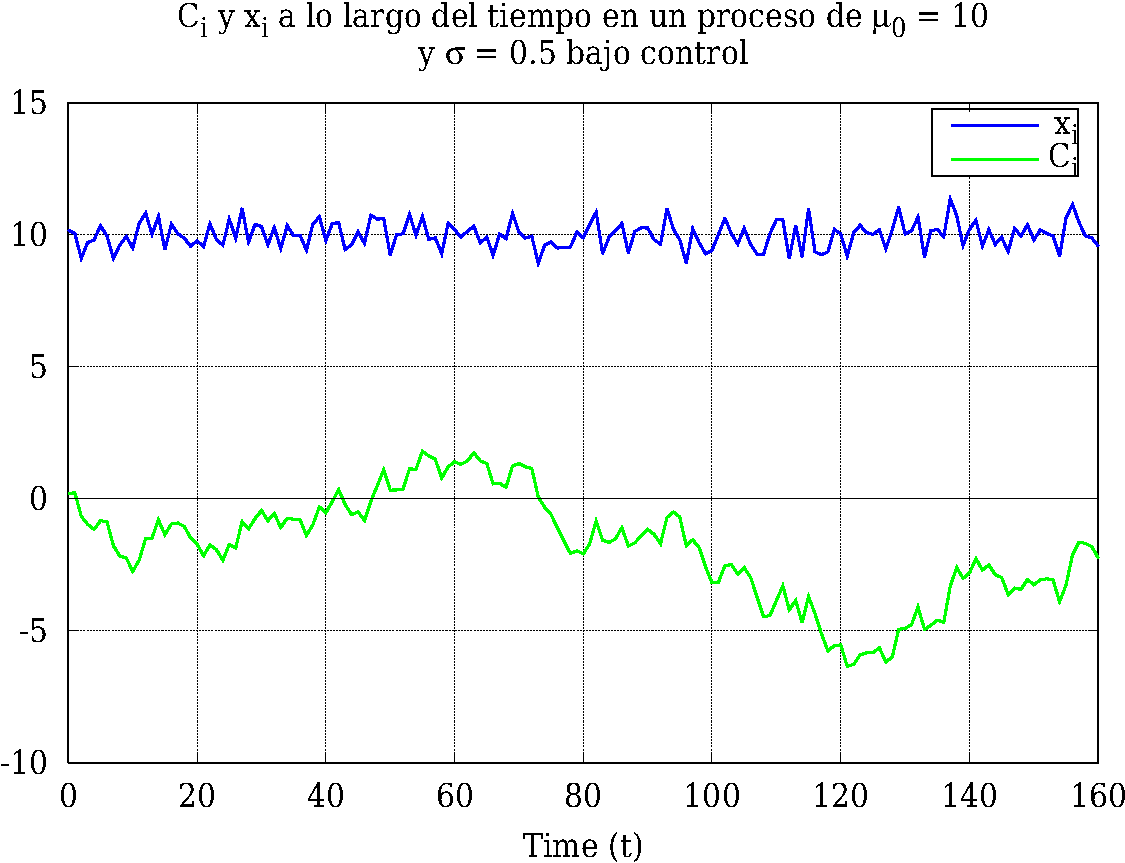
\includegraphics[width=0.9\textwidth]{CapituloCusum/Figuras/ejemploCusumControlado_crop}
\caption{Algoritmo CUSUM aplicado sobre un proceso controlado}
\LABFIG{cusum_controlado} 
\end{figure}
%

\begin{lstlisting}[language=Matlab,caption={Algoritmo CUSUM en procesos bajo control}, breaklines=true, 
label=code:cusum_controlado,numbers=left,float=hbtp]
clear all
close all

N     = 161; % Número de muestras
sigma = 0.5; 
mu    = 10;

x = [0:N-1];
y = mu + sigma*randn(1,N);
z = zeros(1,N);

z(1) = y(1)-mu;
for i=2:N
    z(i) = z(i-1) + (y(i) - mu);
end

plot(x,y,'color','blue','LineWidth',4)
plot(x,z,'color','green','LineWidth',4);
plot([0,N-1],[0,0],'color','black')
axis([0,N-1])
\end{lstlisting}

Para hacernos una idea visual, generamos una gráfica con el código octave \autoref{code:cusum_controlado}, y vemos su 
resultado en la \FIG{cusum_controlado}.

Si el procedimiento está bajo control, vemos cómo $C_i$ oscila en torno al 0, con mayor o menor desviación.

Por su parte, si desajustamos el proceso, y su media comienza a valer $\mathbb{E}(x) = \mu_0 + k$:

\begin{align}
 \mathbb{E}(C_i) &= \mathbb{E}\left[\left(x_1 - \mu_0\right) + \left(x_2-\mu_0\right)+\hdots
                                                                             +\left(x_i-\mu_0\right)\right] \nonumber\\
                 &= \mathbb{E}\left[\sum_{j=1}^i\left(x_j-\mu_0\right)\right]                               \nonumber\\
                 &= \sum_{j=1}^i\mathbb{E}\left(x_j-\mu_0\right)                                            \nonumber\\
                 &= \sum_{j=1}^i\mathbb{E}\left(x_j\right) - \sum_{j=1}^i\mu_0 = i\left(\mu_0 + k\right) - i\mu_0 = ik
                                                                                             \LABEQ{cusum_descontrol}
\end{align}

Se extrae de la \EQ{cusum_descontrol} que $C_i$ seguirá una recta $C_i=ik$ de pendiente $k$. Volvemos a generar una 
gráfica \FIG{cusum_descontrolado} con el código \autoref{code:cusum_descontrolado}.

\begin{figure}[htbp]
\centering
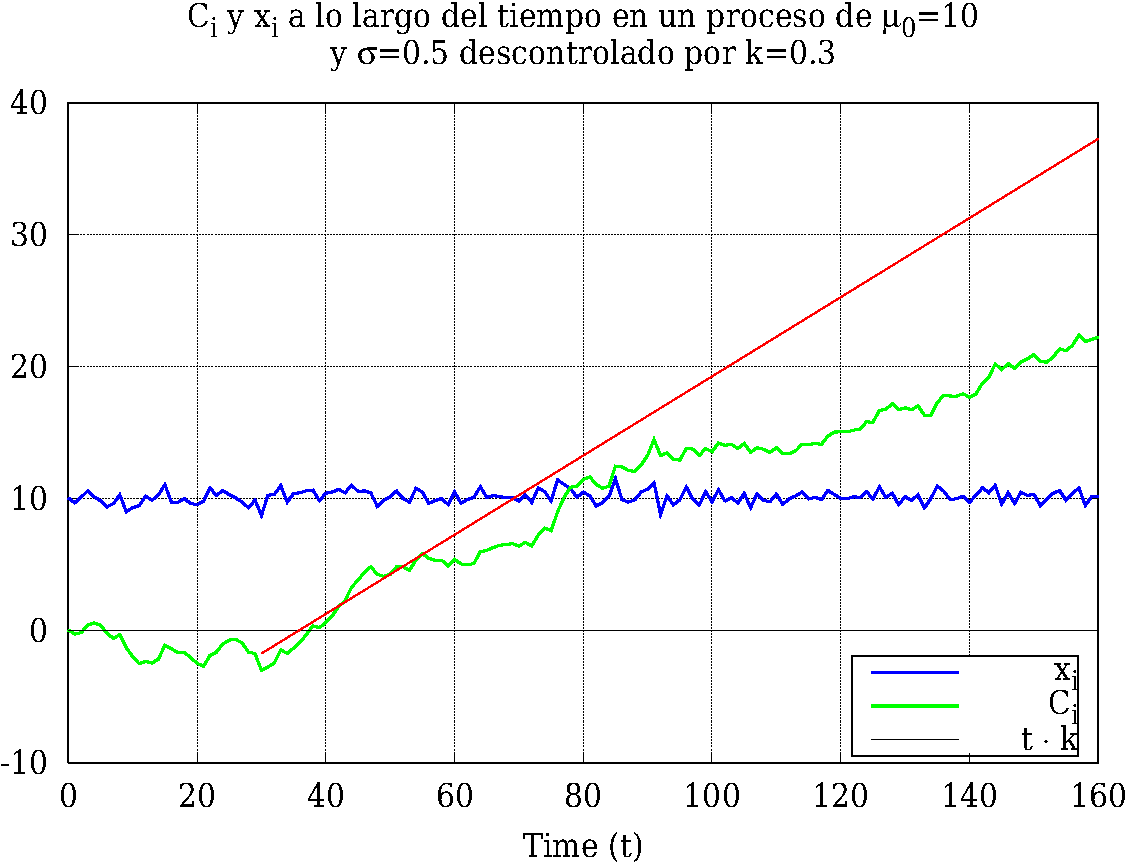
\includegraphics[width=0.9\textwidth]{CapituloCusum/Figuras/cusumDescontrolado-crop}
\caption{Algoritmo CUSUM aplicado sobre un proceso perturbado}
\LABFIG{cusum_descontrolado} 
\end{figure}
%

\begin{lstlisting}[language=Matlab,caption={Algoritmo CUSUM en procesos perturbados}, breaklines=true, 
label=code:cusum_descontrolado,numbers=left,float=htbp]
clear all
close all

N     = 161; % Número de muestras
M     = 30;  % Instante en el que se aplica el descontrol
sigma = 0.5; 
mu    = 10;

x = [0:N-1];
y = mu + sigma*[randn(1,M) k+randn(1,N-M)];
z = zeros(1,N);

z(1) = y(1)-mu;
for i=2:N
    z(i) = z(i-1) + (y(i) - mu);
end

plot(x,y,'color','blue','LineWidth',4)
plot(x,z,'color','green','LineWidth',4);
plot([M,N],[z(M),z(M)+k*(N-M)],'color','red'
plot([0,N-1],[0,0],'color','black')
\end{lstlisting}

Se observa en las figuras que, debido a la extrema sensibilidad que presenta este algoritmo es fácil que el mismo no 
siga la recta predicha en pocas iteraciones. Por eso, el \gls{CUSUM} algorítmico  sólo tendrá en cuenta desviaciones 
que superen un cierto umbral de sensibilidad $K$\index{Umbral de sensibilidad}.

\begin{align}
 C_i^+ &= \max \left[0,\left\{C_{i-1}^+\left(x_i-\mu_0\right)\right\}-K\right] \\
 C_i^- &= \max \left[0,\left\{C_{i-1}^-\left(x_i-\mu_0\right)\right\}-K\right]
\end{align}

Donde $C_i^+$ detecta las desviaciones positivas y $C_i^-$ las negativas.

Es decisión del analista determinar el umbral $K$. Si se quiere detectar un desajuste de $\delta\mu_0=\delta\sigma$,es 
decir, $\mu_1 = \mu_0 + \delta\sigma$ se suele tomar:

\begin{align}
 K = \frac{\delta}{2}\sigma = \frac{\left|\mu_0-\mu_1\right|}{2}
\end{align}

Volvemos a pintar ambas gráficas con el nuevo umbral de sensibilidad en \FIG{cusum_controlado_umbral_sensibilidad} y 
\FIG{cusum_descontrolado_umbral_sensibilidad}, usando \autoref{code:cusum_controlado_umbral} y 
\autoref{code:cusum_descontrolado_umbral}

\begin{figure}[htbp]
\centering
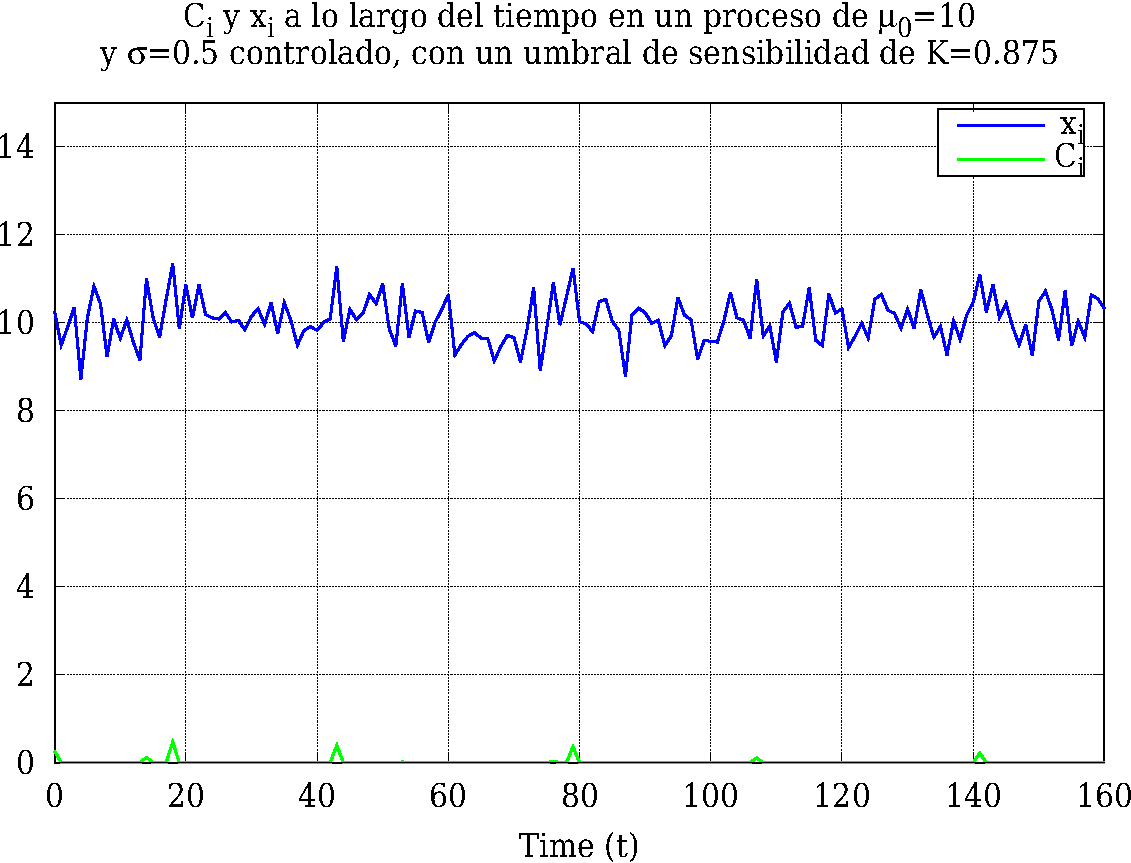
\includegraphics[width=0.9\textwidth]{CapituloCusum/Figuras/cusumControladoUmbral-crop}
\caption{Algoritmo CUSUM aplicado sobre un proceso controlado usando un umbral de sensibilidad}
\LABFIG{cusum_controlado_umbral_sensibilidad} 
\end{figure}
%

\begin{figure}[htbp]
\centering
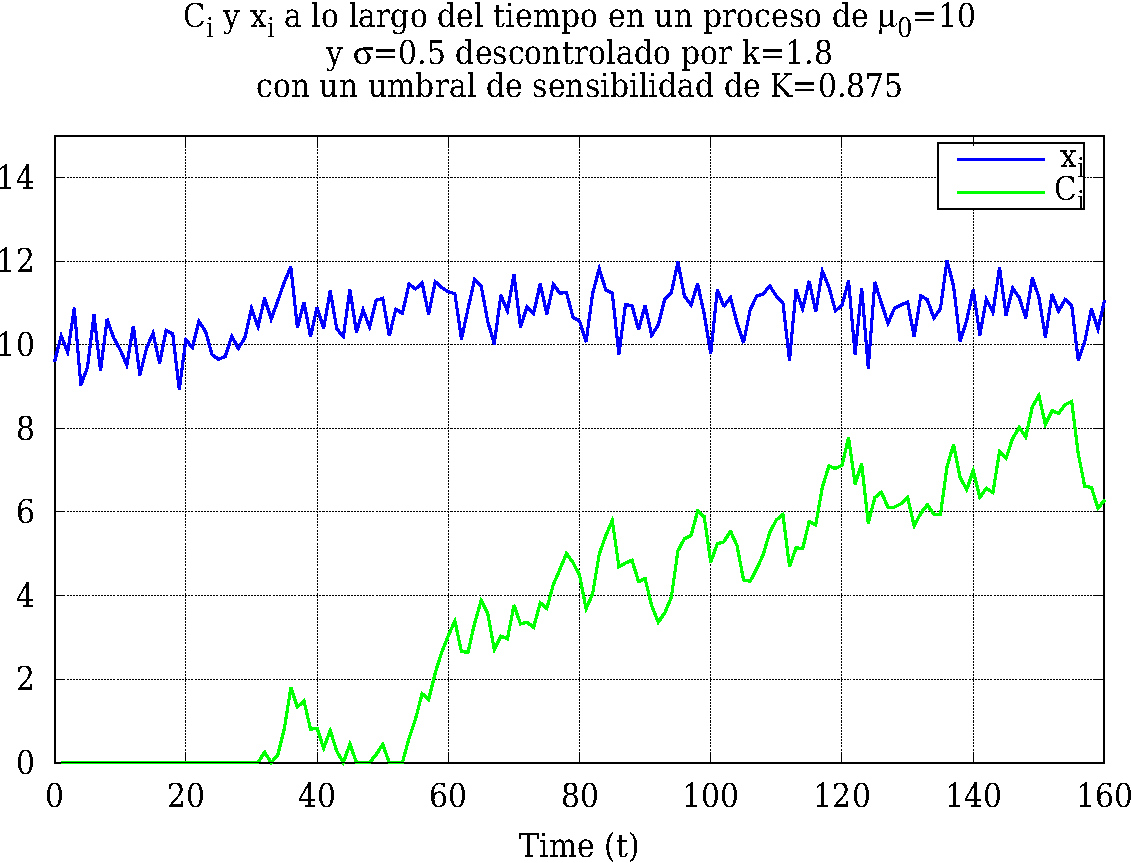
\includegraphics[width=0.9\textwidth]{CapituloCusum/Figuras/cusumDescontroladoUmbral-crop}
\caption{Algoritmo CUSUM aplicado sobre un proceso descontrolado usando un umbral de sensibilidad}
\LABFIG{cusum_descontrolado_umbral_sensibilidad} 
\end{figure}
%

\begin{lstlisting}[language=Matlab,caption={Algoritmo CUSUM en procesos bajo control con umbral de sensibilidad}, 
breaklines=true, label=code:cusum_controlado_umbral,numbers=left,float=htbp]
clear all
close all

N     = 161;        % Número de muestras
M     = 30;         % Instante en el que se aplica el descontrol
sigma = 0.5; 
mu    = 10;
k     = 0;          % Desviación sobre la media
K     = 1.75*sigma; % Umbral de sensibilidad

x = [0:N-1];
y = mu + sigma*[randn(1,M) k+randn(1,N-M)];
z = zeros(1,N);

z(1) = y(1)-mu;
for i=2:N
  z(i) = max(z(i-1) + (y(i) - mu) - K,0);
end

plot(x,y,'color','blue','LineWidth',4)
plot(x,z,'color','green','LineWidth',4);
plot([M,N],[z(M),z(M)+k*(N-M)],'color','red'
plot([0,N-1],[0,0],'color','black')
\end{lstlisting}

\begin{lstlisting}[language=Matlab,caption={Algoritmo CUSUM en procesos perturbados con umbral de sensibilidad}, 
breaklines=true, label=code:cusum_descontrolado_umbral,numbers=left,float=htbp]
clear all
close all

N     = 161;        % Número de muestras
M     = 30;         % Instante en el que se aplica el descontrol
sigma = 0.5; 
mu    = 10;
k     = 1.8;        % Desviación sobre la media
K     = 1.75*sigma; % Umbral de sensibilidad

x = [0:N-1];
y = mu + sigma*[randn(1,M) k+randn(1,N-M)];
z = zeros(1,N);

z(1) = y(1)-mu;
for i=2:N
  z(i) = max(z(i-1) + (y(i) - mu) - K,0);
end

plot(x,y,'color','blue','LineWidth',4)
plot(x,z,'color','green','LineWidth',4);
plot([M,N],[z(M),z(M)+k*(N-M)],'color','red'
plot([0,N-1],[0,0],'color','black')
\end{lstlisting}

Por último, restaría estudiar un umbral de control $H$\index{Umbral de Control}, a partir del cual emitiríamos la 
alarma si $C_i^+$ o $C_i^-$ sobrepasase dicho valor. Generalmente, $H=5\sigma$, pero, de nuevo, depende de la 
sensibilidad del algoritmo el escoger un valor u otro.

\section{Algoritmo CUSUM aplicado al control del tráfico}\index{Control del tráfico}
El tráfico de red es muy dificil de modelar, debido a su naturaleza caótica. Para comenzar, existen muchísimas 
características que podríamos tener en cuenta a la hora de controlar: número de paquetes, paquetes TCP con un bit 
concreto activado\footnote{Esto suma 6 nuevas características}, número de paquetes dirigidos a la misma IP, o desde la 
misma, número de paquetes dirigidos a un servicio particular\footnote{$2^{16}=65536$ posibilidades para TCP y otras 
tantas para UDP}, etc. 

Por otro lado, sean cuales sean los parámetros escogidos, ¿cuáles son sus valores normales? El valor de tráfico normal 
para la página de Slashdot es un ataque de denegación de servicio brutal para las páginas de las noticias que 
enlazan\footnote{Este ataque fue explicado en el \SSSEC{DoS por inundacion}}. Otro elemplos son los denominados 
\emph{Eventos Flash}\index{Eventos Flash}, en los que se produce un incremento de tráfico legítimo \cite{Raghavan}.

En esta sección, describiremos cómo aplicar el algoritmo CUSUM al modelado y caraterización del tráfico: Qué parámetros 
conviene revisa y por qué se han elegido esos (\SSEC{Parametros de interés}), y por qué son neecsarios y cómo debe 
funcionar el sistema de defensa en el periodo de aprendizaje y defensa, así como las aciones que debe tomar si detecta 
que estamos bajo un posible ataque (\SSEC{Periodo de aprendizaje} y \SSEC{Periodo de defensa}).

\subsection{Parámetros de interés}\LABSSEC{Parametros de interés}
S.V. Raghvan y E.Dawson señalan los siguientes como los parámetros más importantes a la hora de detectar un ataque 
\gls{DoS}:

\begin{itemize}
 \item \gls{OWCD}, Densidad de conexiones de un solo sentido
 \begin{align}
  \text{OWCD} = \frac{\sum\text{Paquetes OWC}}{\sum\text{Paquetes IP}}
 \end{align}

 \item Longitud media de paquetes.
 \begin{align}
  <L>_{\text{flow}} = \frac{\sum\text{Paquetes IP}}{\sum\text{Flujos IP}}
 \end{align}
 
 \item Relación paquetes entrantes y salientes
 \begin{align}
  R_{io} = \frac{\sum\text{Paquetes entrantes}}{\sum\text{Paquetes salientes}}
 \end{align}
 
 \item Porcentaje de paquetes TCP
 \begin{align}
  R_{io} = \frac{\sum\text{Paquetes TCP}}{\sum\text{Paquetes IP}}
 \end{align}
 
 \item Porcentaje de paquetes UDP
 \begin{align}
  R_{io} = \frac{\sum\text{Paquetes UDP}}{\sum\text{Paquetes IP}}
 \end{align}
 
 \item Porcentaje de paquetes ICMP
 \begin{align}
  R_{io} = \frac{\sum\text{Paquetes ICMP}}{\sum\text{Paquetes IP}}
 \end{align}
 
 \item Porcentaje de paquetes LAND, esto es, que tienen la misma dirección IP origen y destino
 \item Tipo de potocolo: \gls{TCP}, \gls{UDP}, \gls{ICMP}... 
\end{itemize}

Para la obtención de dichos parámetros, se monitorizará el tráfico desde y hacia el activo protegido por cada IP 
externa\footnote{Más adelante definiremos el concepto de \gls{IP} externa, en la sección \ref{TODO}. Por ahora, se 
trata de la \gls{IP} que intenta acceder al activo defendido, o a la que el activo defendido está respondiendo.}, 
acumulando los bytes y paquetes por protocolo, bytes y paquetes entrantes y salientes, el conteo de los paquetes LAND, 
los paquetes \gls{TCP} \gls{SYN} y aquellos marcados con los bits \gls{SYN} y \gls{ACK} al mismo tiempo. 

Tras intervalos de tiempo regulares, se extraerá de ese conteo los parámetros enumerados anteriormente, lo que supondrá 
una muestra de cada estadístico por cada IP, más una muestra global.

Según los datos aprendidos a lo largo del tiempo, y los datos que aprendamos en este intervalo de tiempo, el programa 
puede estar en estado \emph{Aprendizaje}, en estado \emph{Defensa} o en estado \emph{Alarma} (ver 
\FIG{diagrama_estados}). En qué consiste cada estado, y las causas de las transiciones se encuentran en las siguiente 
secciones.

\begin{figure}[htbp]
\centering
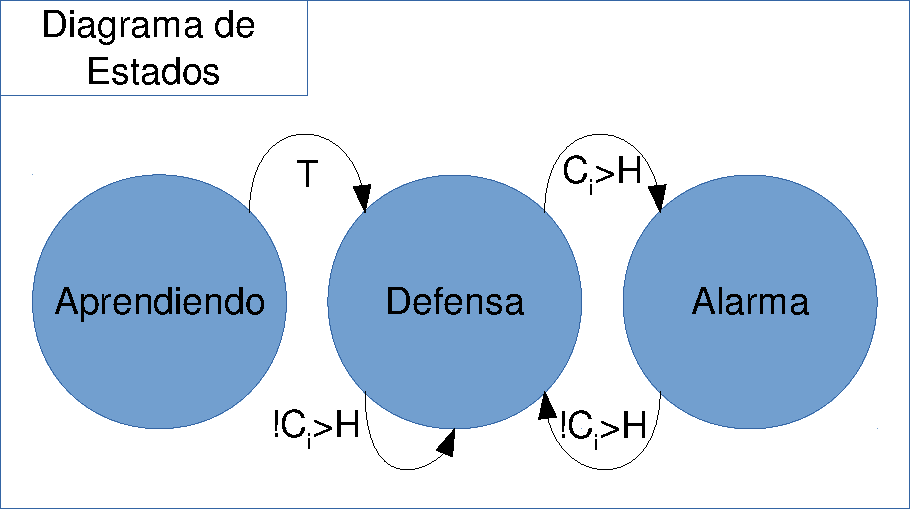
\includegraphics[width=0.6\textwidth]{CapituloCusum/Figuras/DiagramaEstados-crop}
\caption{Diagrama de estados del sensor}
\LABFIG{diagrama_estados} 
\end{figure}
%

\subsection{Periodo de Aprendizaje}\LABSSEC{Periodo de aprendizaje}\index{Periodo de Aprendizaje}
Para poder aplicar el algoritmo CUSUM, es necesario conocer la media y la desviación cuadrática de cada parámetro en el 
tráfico que estamos analizando. Sin embargo, como ya hemos dicho en la introducción de esta sección, es imposible saber 
a priori qué media o qué desviación deben tener dichos parámetros. Se hace necesario un periodo de aprendizaje, en el 
que extraigamos del tráfico dichos estadísticos.

En este periodo de aprendizaje el sistema de defensa recopila la información descrita en la 
\SSEC{Parametros de interés}, y realiza cada intervalo de tiempo $T$ un muestreo. Tras $N$ intervalos, se puede sacar 
una media $\mu_0$ y una desviación cuatrática $\sigma$ del valor que deben tener dichos parámetros.

Es obligatorio suponer que, durante el periodo de aprendizaje, no ha habido ningún ataque realizado sobre la red 
protegida. De cometerse un ataque sobre la red, este será el tomado como \emph{normal} o \emph{típico}, y las 
características del tráfico legítimo no coincidirán.

Una posible forma de conseguir esto podría ser capturar tráfico en un fichero \gls{PCAP}, comprobar que esté libre de 
ataques, y hacerlo pasar por el sistema de aprendizaje. Tras ello, Se extraerá la media y la desviación típica de dicho 
periodo, y se podrá comenzar con el periodo de defensa.

\subsection{Periodo de defensa}\LABSSEC{Periodo de defensa}\index{Periodo de Defensa}
Tras el periodo de aprendizaje (ver \SSEC{Periodo de aprendizaje}), tenemos unos estadísticos con los que comparar el 
tráfico. Por tanto, podemos detectar ataques: Decimos que estamos en el periodo de defensa.

El funcionamiento básico será el mismo que en el periodo de aprendizaje: Por cada \gls{IP}, registramos los valores 
anteriormente descritos. Tras un intervalo de tiempo, extraemos los parámetros significativos enumerados.

Sin embargo, ahora sí poseemos una media y desviación típica con la que comparar. Por tanto, es posible definir un 
valor $C_{i,\text{IPexterna}}$ para cada parámetro, IP externa e intervalo de tiempo, que permita decidir si estamos o 
no bajo ataque por alguna IP concreta. Por otra parte, se lleva la cuenta de estas características a nivel general, por 
lo que también se podrán detectar ataques realizados a base de clonar el comportamiento normal en muchas direcciones 
\gls{IP} distintas.

Si se produce una alarma, esto es, $C_{i,\text{IP}} > H$ para alguna \gls{IP} o los contadores generales, se pasará al 
Modo Alarma\index{Modo Alarma}\index{Modo Alarma}. 

\subsubsection{El aprendizaje durante el periodo de defensa}

Durante el periodo de defensa, es necesario seguir aprendiendo. Por ejemplo, si la media da un valor bajo para los 
paquetes \gls{UDP}, y un cliente sólo se dedica a hacer consultas \gls{UDP} legítimas, es posible que este alcance muy 
pronto el valor umbral para el ratio \gls{UDP}, lo que provocaría una falsa alarma. Por tanto, ante cada nueva IP de la 
que se tengan datos, será necesario hacerla pasar por un tramo de aprendizaje, de forma que se pueda comparar consigo 
misma a lo largo del tiempo.

Por otra parte, si el periodo de aprendizaje ha caído en una hora valle del tráfico, el funcionamiento normal será 
identificado rápidamente como un ataque. Así pues, tras el periodo de aprendizaje original, se realizará otro periodo 
de aprendizaje provisional. Si no se producen alarmas durante este periodo, los nuevos valores \emph{normales} pasarán 
a ser los aprendidos.

\subsubsection{Protocolo de actuación ante un ataque. Modo Alarma}

Ante un ataque, podríamos actuar de tres formas distintas \cite{Raghavan}:
\begin{enumerate}
 \item\emph{Detener el tráfico atacante}, aceptando el riesgo de detener también tráfico legítimo.
 \item\emph{Frenar el tráfico atacante}, lo cual requiere una capacidad de procesamiento mayor por parte del sistema de 
filtrado, que podría llevar a una respuesta mas lenta.
 \item\emph{Aprovisionamiento de recursos}, lo cual puede o puede no ser posible en ese momento.
\end{enumerate}

De las anteriores opciones, la más usada es la de frenar completamente el tráfico considerado como atacante, ya que es 
la que estamos seguros que siempre se podrá llevar a cabo sin afectar negativamente al rendimiento.

Así pues, ante un ataque, el primer paso será dejar de admitir flujos provenientes de direcciones \gls{IP} que no 
hayan sido previamente registradas, de forma que se reduzca el flujo de información hacia el servidor. Esto puede dejar 
fuera conexiones legítimas, pero el permitir nuevas conexiones podría ser aprovechable para continuar machacando el 
servicio.

Tras ello, es necesario inspeccionar, si las hubiese, qué flujos \gls{IP} han ocasionado que salte la alarma, mediante 
el algoritmo \gls{CUSUM} aplicado a cada uno. Se seguirán deteniendo los flujos hasta que, mediante el algoritmo 
\gls{CUSUM} de nuevo, se detecte que estamos fuera de la zona de alerta.

\section{Resumen}%%%%%%%%%%%%%%%%%%%%%%%%%%%%%%%%%%%%%%%

\begin{Resumen}[Resumen del capítulo]
\subsection*{El algoritmo CUSUM}
\begin{displaymath}
\begin{cases}
 \text{control de procesos}
 \begin{cases}
  \text{Diferencia las las pautas \emph{normales} y las \emph{desviaciones}}\\
  \text{Diferencia procesos \emph{bajo control} y \emph{fuera de control}}   \\
  \text{Podemos usarlo para distinguir tráfico legítimo del atacante}
 \end{cases}\\\\

 \text{CUSUM}
 \begin{cases}
  \text{-- SCP con memoria: Detecta pequeñas variaciones a lo largo de mucho tiempo} \\ 
  \qquad x_1,x_2,x_3... \Rightarrow f(x_1),f(x_1,x_2),f(x_1,x_2,x_3)... \\
  \qquad C_1 = (x_1 - \mu_0) \\
  \qquad C_i = C_{i-1} + \left(x_i-\mu_0\right) \\
  \text{-- Se le añade un umbral de sensibilidad $K = K(\sigma)$}\Rightarrow\text{Cambios pequeños no afectan} \\
  \qquad C_i^+ = max\left[0, C_{i-1} + \left(x_i-\mu_0\right)- K\right]\\
  \qquad C_i^- = max\left[0, C_{i-1} - \left(x_i-\mu_0\right)- K\right]\\
  \text{-- Alarma si $C_i$ supera un valor $H = H(\sigma)$} \\
 \end{cases}
\end{cases}
\end{displaymath}

\subsection*{Cusum aplicado al control del tráfico}
\begin{displaymath}
 \begin{cases}
  \text{Parámetros de interés}
  \begin{cases}
   \text{Densidad de conexiones en un sentido} \\
   \text{Longitud media de paquetes} \\
   \text{Relación entre paquetes entrantes y salientes} \\
   \text{Porcentaje de paquetes \gls{TCP}} \\
   \text{Porcentaje de paquetes \gls{UDP}} \\
   \text{Porcentaje de paquetes \gls{ICMP}} \\
   \text{Porcentaje de paquetes LAND (ip origen = ip destino)}
  \end{cases}\\\\
  \text{Periodo de aprendizaje}
  \begin{cases}
   \text{Necesario debido a que no conocemos $\mu_0$ ni $\sigma$ del tráfico} \\
   \text{Acumulación de muestras para conocer dichos parámetros durante un tiempo} \\
   \text{Se supone que no han habido ataques durante el periodo de aprendizaje}
  \end{cases}\\\\
  \text{Periodo de defensa}
  \begin{cases}
   \text{Aplicamos el algoritmo \gls{CUSUM} al tráfico analizado} \\
   \text{Si alguna \gls{IP} o los contadores generales superan $H$, se entra en modo defensa} \\
   \text{Modo defensa}
   \begin{cases}
    \text{Bloqueo de nuevas \gls{IP}} \\
    \text{Búsqueda y bloqueo de IP maliciosas ($C_{i,\text{IP}} > H$).}
   \end{cases}
  \end{cases} \\
 \end{cases}
\end{displaymath}


\end{Resumen}

